\subsection{UX Diagram}
As a way to show the navigation among the different pages and define the visual flow of screens we redesigned a completed User Experience diagram starting from the draft that was introduced in the RASD document.

\begin{center}
\begin{figure}[htp] 
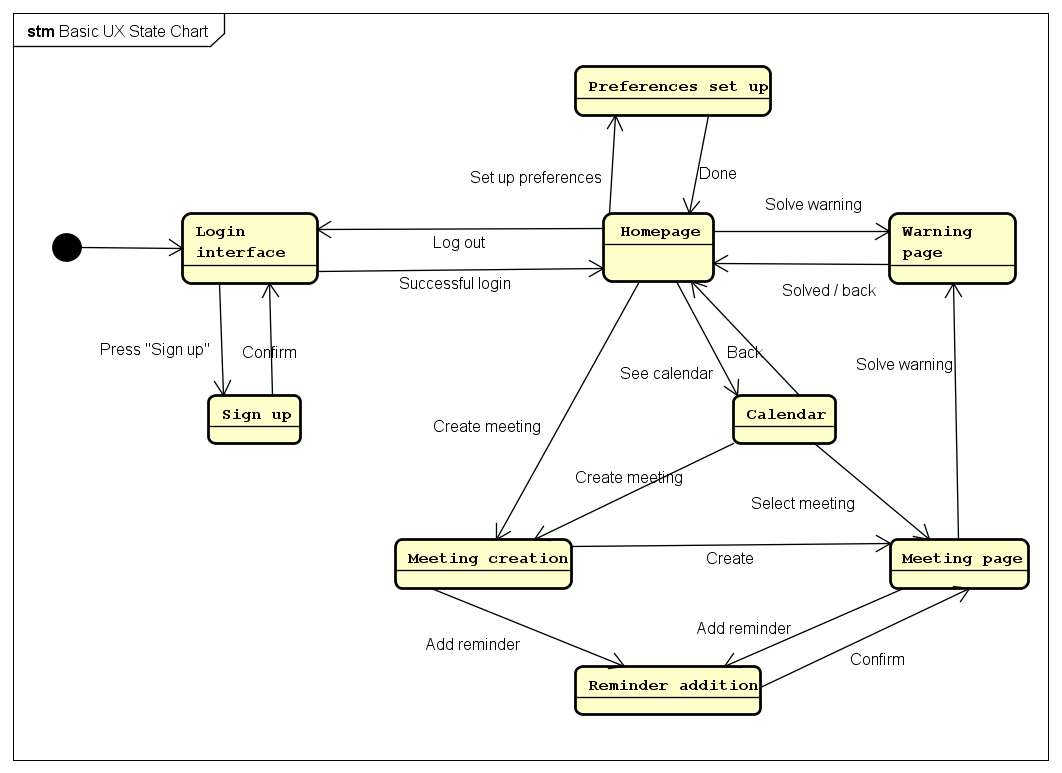
\includegraphics[width=\textwidth]{images/basicux} 
\caption{The initial UX diagram} 
\label{fig:basicux} 
\end{figure} 
\end{center}





\begin{figure} 

\begin{center}

\makebox[\textwidth]{%
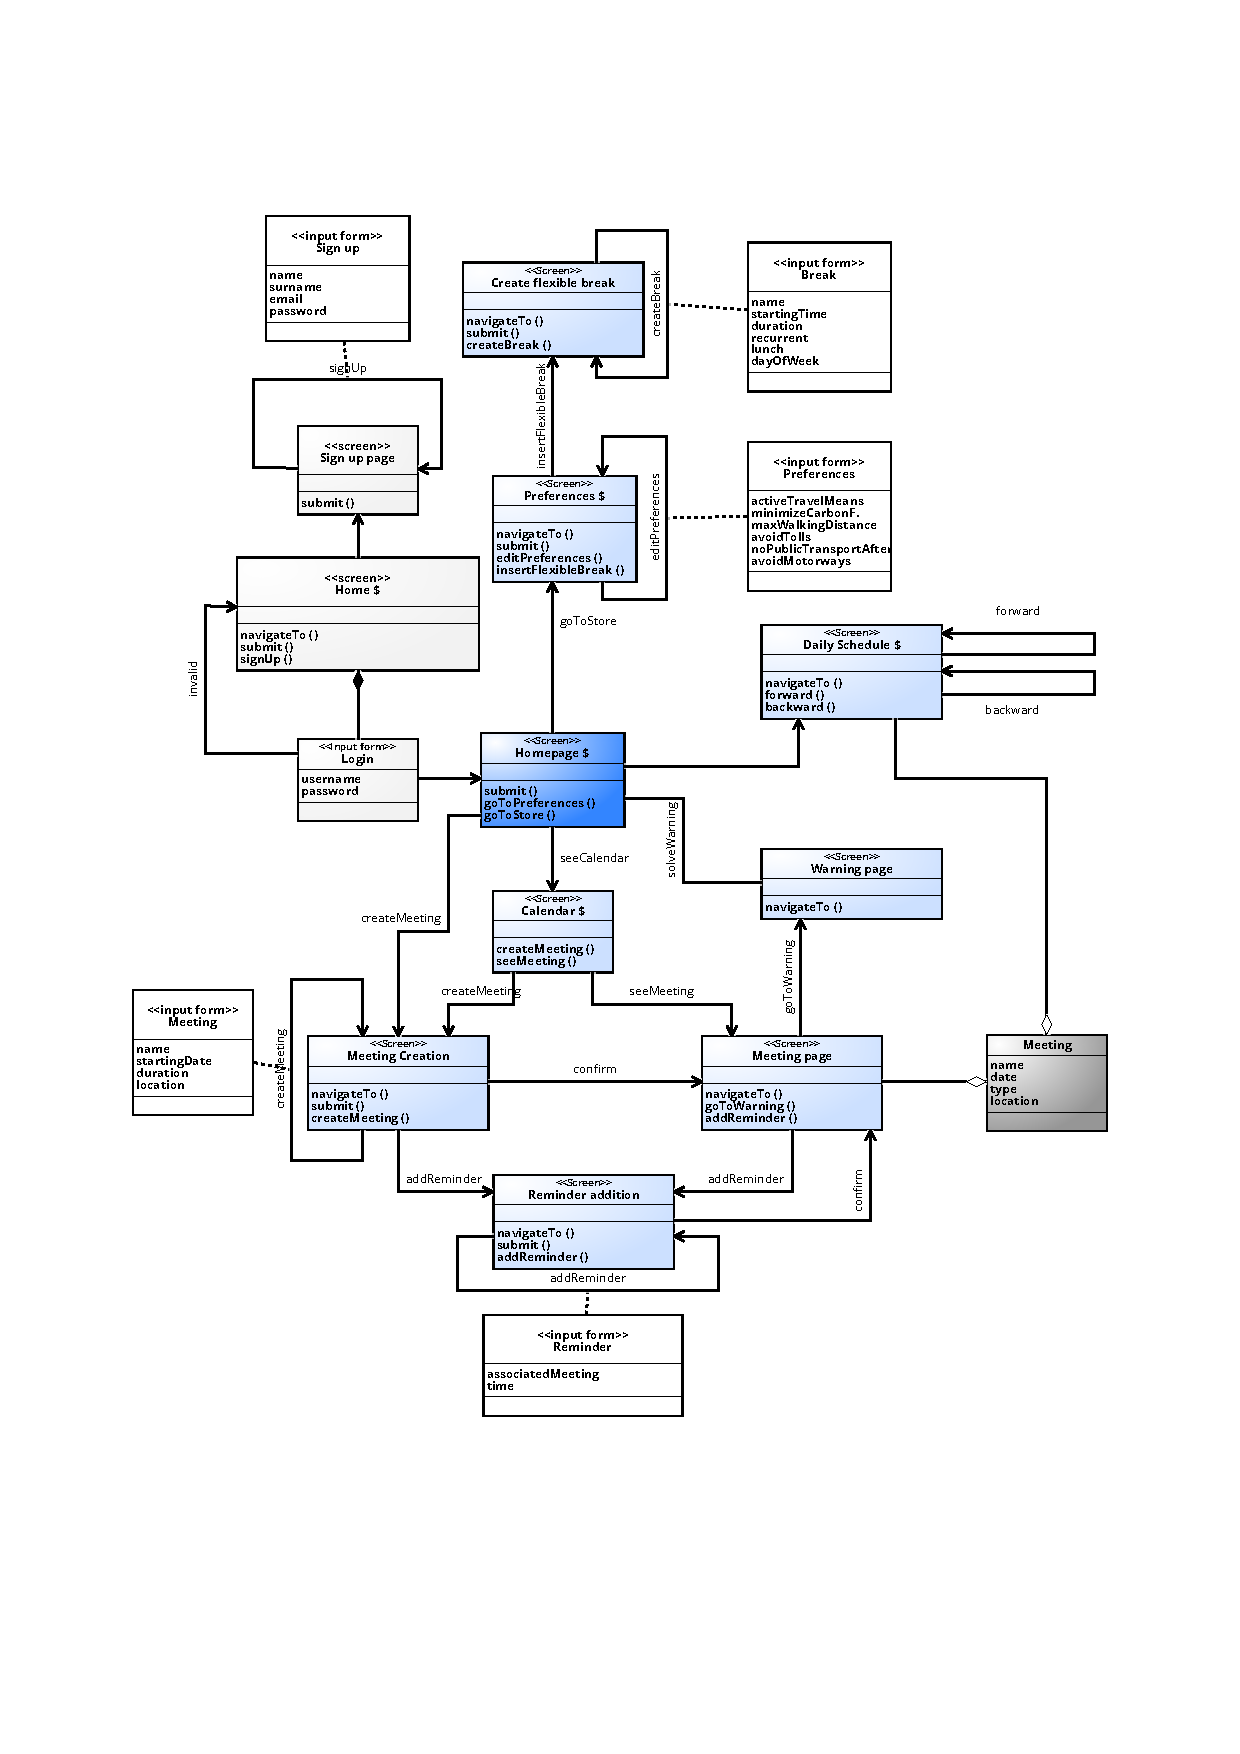
\includegraphics[width=1.4\linewidth]{images/completeuxtravlendar} 
}
\caption{The complete User Experience diagram of the application} 
\label{fig:ux} 


\end{center}
\end{figure} 


\clearpage

\subsection{Mockups of the User Interface}
	\begin{flushleft}
		Concerning the user interface requirements, we established to directly provide information about the application screens and layout through several mockups. \\
		We designed the sketch of the main pages of Travlendar+ following our aim to make a light and user friendly product but, at the same time, we have pursued an attractive and impressive style. \\
		Apparently, the coding phase could affect our desing. Hence, these sketches are not definitive, their aim is to give an idea of the application design. \\
		For this reason, if we notice that some changes are necessary due to either app. improvement or obstacles in realization, we would be ready to modify them. 
	\end{flushleft}
\clearpage

	\begin{figure}
			\begin{flushleft}
			\subsubsection{Homepage}
			To pursue our aim of realizing a user-friendly and light app, we decided to provide the main functions directly in the homepage. Indeed, from this page, a guest can reach the sign up form, a user can log himself in,can insert a meeting by tapping onto a day in the calendar,can manage his preferences and even access the warnings. \\ 
		\end{flushleft}
		\centering
		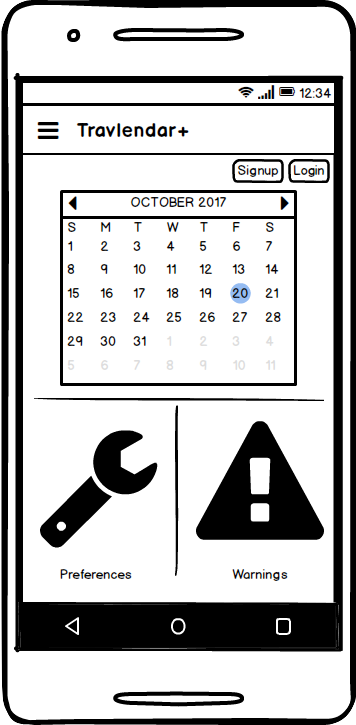
\includegraphics[width=0.6\linewidth]{mockups/Homepage}
		\caption{Travlendar+ homepage.  
		}
	\label{fig:homepage}
	\end{figure}

	\begin{figure}
			\begin{flushleft}
			\subsubsection{Quick Menu}
			We thought about a quick menu to collect some secondary functions, to make them easily reachable. By tapping on the top-left corner of the app people have the opportunity to either register or log in themselves, to only view meetings of the current day, to access the reminders they set up, to manage the warnings and to logout if they are already logged in.
		\end{flushleft}
	\centering
	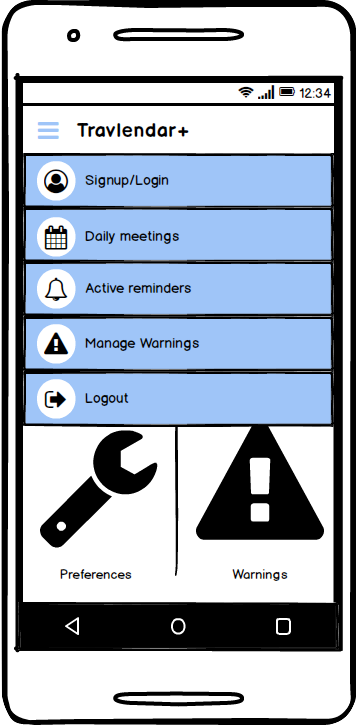
\includegraphics[width=0.6\linewidth]{mockups/QuickMenu}
	\caption{Quick access menu.}
	\label{fig:quickmenu}
	\end{figure}
\clearpage

	\begin{figure}
			\begin{flushleft}
			\subsubsection{Meeting Creation}
			This page is a very simple form, which allows the user to finalize the creation of a meeting by filling it in all its fields. 
			The house-logo in the  right corner,on the top band and near the application name, represents the return-to-homepage icon. 
		\end{flushleft}
		\centering
		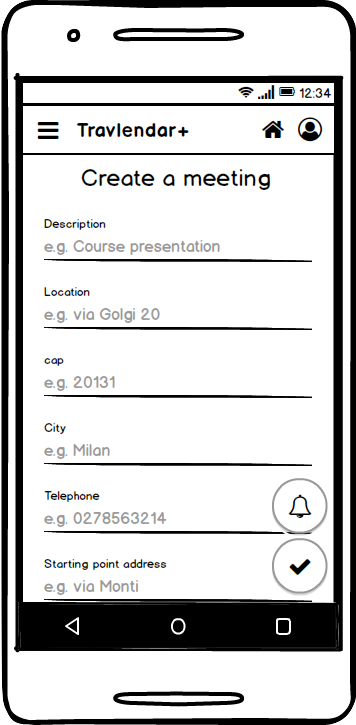
\includegraphics[width=0.6\linewidth]{mockups/CreateMeeting}
		\caption{Meeting creation page.}
		\label{fig:createmeeting}
	\end{figure}

	\begin{figure}
			\begin{flushleft}
			\subsubsection{Meeting Page}
			This screen wants to provide all the useful information related to a meeting already registered in the system. First details provided, in the highest portion of the page, regard the meeting location and the route to reach the appointment, further information are located below. In addition, on the right part of the screen, there are quick access buttons: the "plus" icon allows the user to add a reminder for the event, the "pencil" icon is to change meeting details and the "x" button provides deletion function. 
		\end{flushleft}
	\centering
	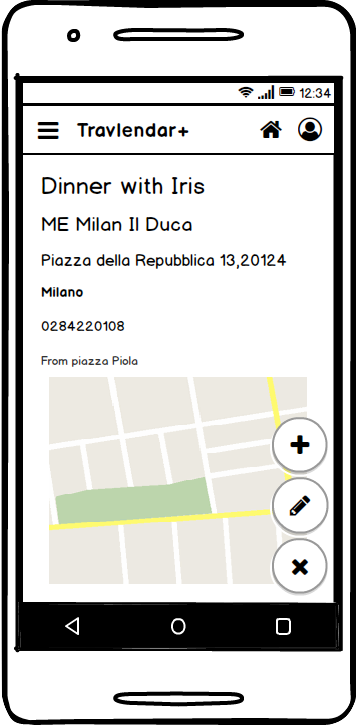
\includegraphics[width=0.6\linewidth]{mockups/MeetingView}
	\caption{Meeting view page. }
	\label{fig:meeting-view}
	\end{figure}
\clearpage

	\begin{figure}
			\begin{flushleft}
			\subsubsection{Warning Page}
			The warnings page has the role to summarize and notify all the conflicts among meetings which involve the user's appointments. Every warning is represented by a dialog which points out the meetings that generate the conflict and which has two buttons, one to ignore the warning and other one to solve it by modifying the conflictual meetings. 
			To prevent too much user's clicks, an "ignore all" button is provided, which is equivalent to tap "ignore" for each warning in the list. 
		\end{flushleft}
		\centering
		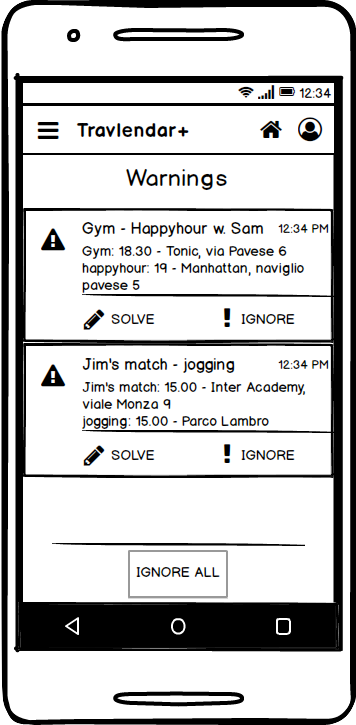
\includegraphics[width=0.6\linewidth]{mockups/Warnings}
		\caption{Warnings page}
		\label{fig:warnings}
	\end{figure}
\clearpage

	\begin{figure}
				\begin{flushleft}
				\subsubsection{Travel means preferences}
			This is a very simple page with a minimalistic design, not to uselessly load the application. However, this basical view provides all the functions which the user needs to select his preferences related to the transports for his travels. 
			Please notice that the preferences section can be changed by tapping on an specific topic just below the "Preferences" bar.
		\end{flushleft}
		\centering
		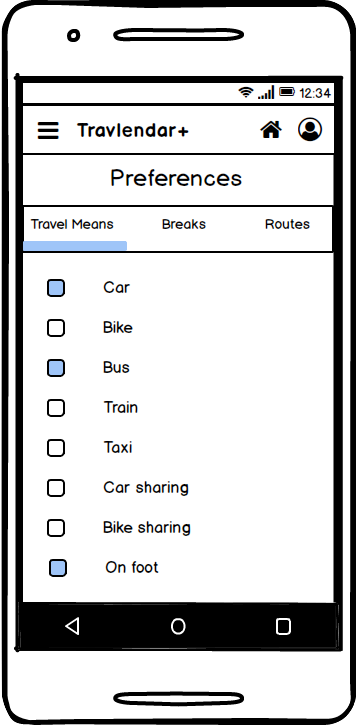
\includegraphics[width=0.6\linewidth]{mockups/PreferencesTravelMeans}
		\caption{Travel mean preferences page.}
		\label{fig:preferencestravelmeans}
	\end{figure}

		\begin{figure}
				\begin{flushleft}
				\subsubsection{Breaks preferences}
				The breaks page consists in a list of events, that represent pauses, organized in order of creation and labeled by the type of the break. For every break  both the starting and the ending time, a "pencil" button to allow modifications and a "x" button,to remove it, are provided. In addition, thanks to the fact that we decided to make the breaks general, that means not related to a specific day, the user has the faculty to either flag or unflag them to activate or deactivate them. 
			\end{flushleft}
		\centering
		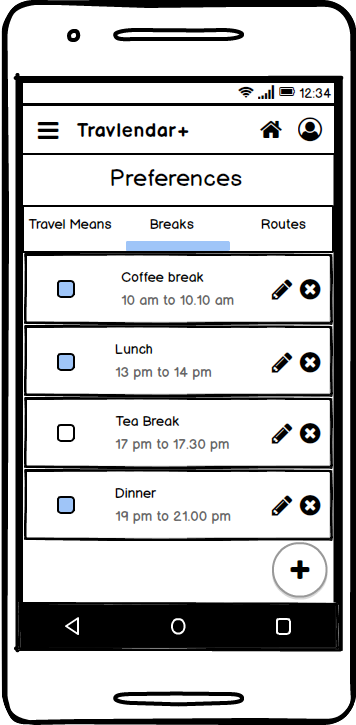
\includegraphics[width=0.6\linewidth]{mockups/PreferencesBreaks}
		\caption{Break preferences page.}
		\label{fig:preferencesbreaks}
	\end{figure}
	
		\begin{figure}
				\begin{flushleft}
				\subsubsection{Route preferences}
				The route preferences page is very similar to the Travel mean preferences page. The style is the same and the opportunity to flag or unflag elements too, however there are differences. Some of the preferences in this section are mutal exclusive, so the user is prevented to select more than one of them (for instance a user can select either the shortest route or the fastest). Moreover, some selection element has customizable details, they are represented with a pencil logo on the right, and can be managed by the user to best fit his preferences (for example the user can select after which hour he does not want to use public transportations).
			\end{flushleft}
		\centering
		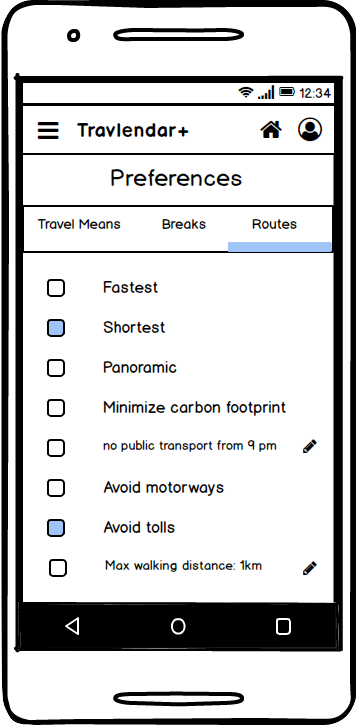
\includegraphics[width=0.5\linewidth]{mockups/PreferencesRoutes}
		\caption{Route preferences page}
		\label{fig:preferencesroutes}
		
	\end{figure}
	